\documentclass{subfiles}

\begin{document}
    \subsection*{Versuchsprotokoll} 
        \marginnote{Start 9:20}
        Wir einigen uns auf den Ordnernamen 
        \begin{center}
            \texttt{C://Users/fpphysik/Desktop/Daten/WiSe23-24/Tiwary-Jannack-Folgmann/}
        \end{center}
        und sortieren in Unterordnern \texttt{./i} für $i$ als Versuchsdurchführungsnummer. Als Test nehmen wir die in \ref{fig:TestPulseAndCollect} dargestellten folgenden Parameter auf:
        \begin{figure}[H]
            \centering
            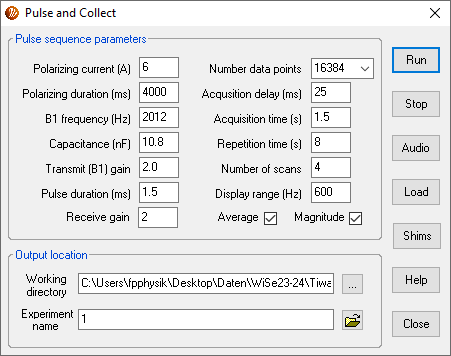
\includegraphics[width=5cm]{Live-Dokumente/Bilder/Testaufnahme-Pulse-And-Collect.PNG}
            \caption{Testaufnahme der \enquote{Pulse and Collect} Parameter.}
            \label{fig:TestPulseAndCollect}
        \end{figure}

        \paragraph*{Versuchsteil 2}
            Der Live-Plot der \texttt{Exp1} Messreihe (siehe Tabelle unten) ist gegeben durch:
            \begin{figure}[H]
                \centering
                \begin{subfigure}[b]{0.4\textwidth}
                    \centering
                    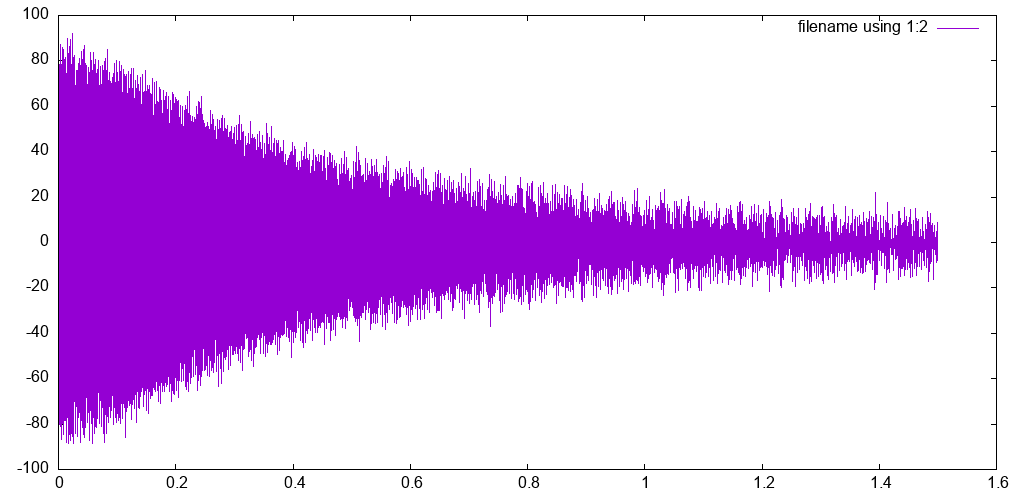
\includegraphics[width=5cm]{Live-Dokumente/Bilder/Exp1_FID.png}
                    \caption{FID.}
                \end{subfigure}
                \
                \begin{subfigure}[b]{0.4\textwidth}
                    \centering
                    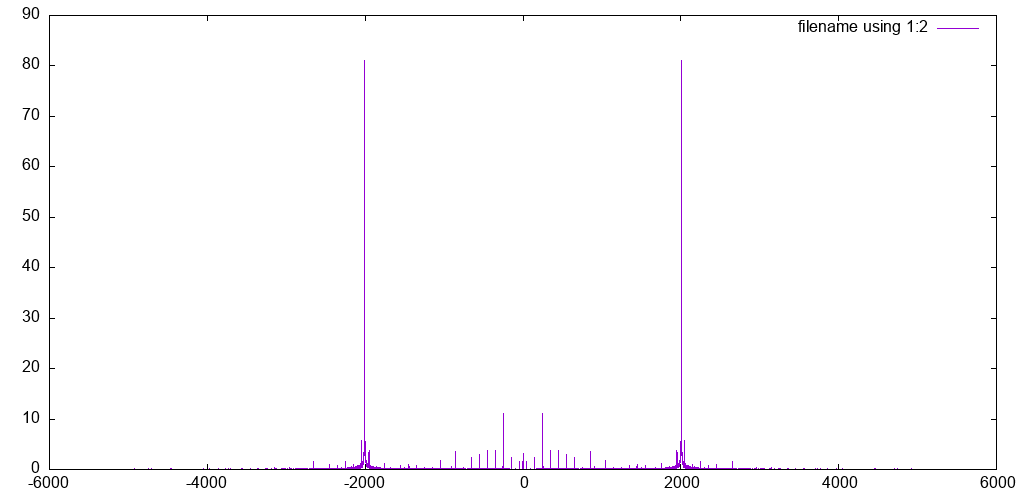
\includegraphics[width=5cm]{Live-Dokumente/Bilder/Exp1_Spectrum.png}
                    \caption{Spektrum.}
                \end{subfigure}
                \caption{Live-Plot der \texttt{Exp1} Messreihe.}
                \label{fig:LivePlotExp1}
            \end{figure}
            Wir sehen weiter Dateien mit der Erweiterung \texttt{.1d}. Um diese zu öffnen, betrachte unter \href{https://afni.nimh.nih.gov/afni/community/board/read.php?1,160269,160270}{afni.nimh.nih.gov} die Möglichkeit 
\begin{lstlisting}{language=python}
import lib_afni1D.py as LAD

my_dat = LAD.Afni1D(filename)
\end{lstlisting}


        \paragraph*{Versuchsteil 3}
            Wir sind uns unsicher, was die Aussage des Rauschens ist. 

        \paragraph*{Versuchsteil 4}

            
        \paragraph*{Versuchsteil 5}
            Wir wählen bei \enquote{Autoshim} die angegebenen Parameter. Wir erhalten dieselben Werte wie in \ref{fig:TestPulseAndCollect}, die Parameter waren also bereits optimal. \\

            Wir erhalten nicht die gewünschte Kurve. Man erkennt die Lamorfrequenz als Peak im Zentrum, vermisst allerdings die Resonanzfrequenz des LC-Schwingkreises. Die Lösung besteht darin, den Wert von \emph{aquisation delay} auf $2\si{\ms}$ zu setzen. Zusätzlich setzen wir \emph{diplay range} auf $500\si{\hertz}$. \\

            Bei der $C$ Optimierung stellen wir einen bereits optimalen Wert von $10.8\si{\nano\farad}$ fest. \\

            Bei der $B_1$ Optimierung betrachten wir den Parameter unter \emph{pulse duration}. Wir stellen $1.5\si{\seconds}$ als bereits optimiert fest, wählen nach Inspektion des FID Amplitudengraphen allerdings $1.7\si{\s}$ aus. Die finalen Werte für den Ordner \texttt{B1-Opti} sind damit:
            \marginnote{Ordnerbackup 11:00}
            \begin{figure}[H]
                \centering
                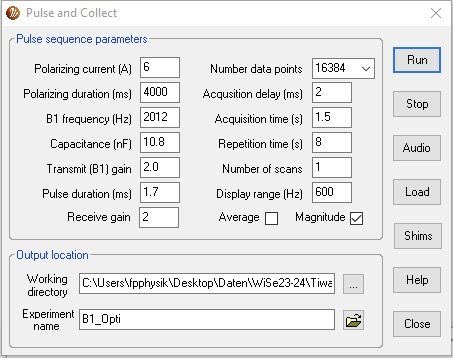
\includegraphics[width=5cm]{Live-Dokumente/Bilder/B1OptiWerte.jpeg}
                \caption{Parameter für die $B_1$ Optimierung (vor Fußnote).}
                \label{fig:B1OptiParam}
            \end{figure}
            \marginnote{Fußnote gelesen 11:15}
            Aufgrund experimenteller Einschränkungen wählen wir ein Vielfaches von $0.5\cdot (1/2012\si{\hertz})\approx 0.248\si{\s}$ aus und verwenden $1.75\si\s$.  


        \paragraph*{Versuchsteil 7}
            Wir erzeugen mit den als optimal erkannten Parametern eine FID und ihre Fouriertransformierte in \texttt{FID-Characterize1}.
            

        \paragraph*{Versuchsteil 8}
            Wir wählen das Polarisationsfeld mit $4$ nacheinanderfolgenden Scans und dem Mittelwert als Ergebnis. 
            \marginnote{Backup Ordner und Log 11:31}
            Als Ergebnisse der $10$ Schritt Messung haben wir die Relaxionszeit $T_1$ als folgenden Graphen.
            \begin{figure}[H]
                \centering
                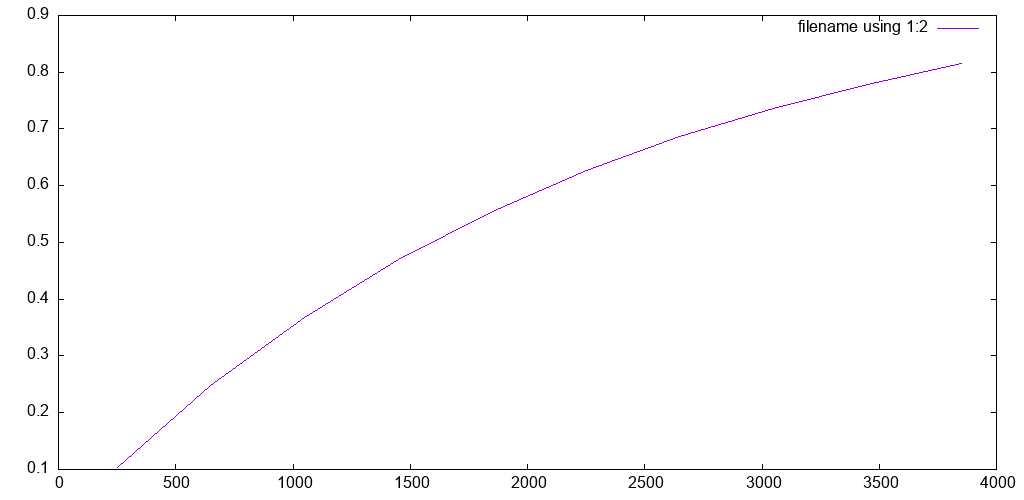
\includegraphics[width=5cm]{Live-Dokumente/Bilder/B1-10steps/T1.png}
                \caption{Amplitude $E/E_0$ über der Zeit $t$ der Polarisierungsdauer.}
                \label{fig:T1}
            \end{figure}

        \paragraph*{Dateinamen}

        \begin{table}[H]
            \centering
            \begin{tabular}{c|c|l[4cm]}
                \textbf{Dateiname} & \textbf{Nutzbarkeit} & \textbf{Bedeutung} \\
                \hline\hline
                \texttt{Exp1} & & \\
                \texttt{Exp2} & & \\
                \hline
                \texttt{AutoShim1} & x & Testlauf des \emph{auto-shimming} \\
                \texttt{AutoShim2} & & \\
                \hline
                \texttt{Explore-FID1} & & Testaufnahme unter Varrierung von \emph{recieve gain} \\
                \texttt{Explore-FID2} & & \\
                \texttt{Explore-FID3} & & \\
                \hline
                \texttt{C-Opti} & x & Wert $10.8$ war bereits optimiert. \\
                \hline
                \texttt{B1DurationFast} & & \\
                \texttt{B1Opti} & & \\
                \hline
                \texttt{FID-Characterize1} & x & Optimale Einstellungen mit \emph{pulse duration} auf $25\si{\ms}$\\
                \texttt{FID-Characterize2} & & \\
                \hline
                \texttt{T1-Bp-10steps} & & Spin-Gitter-Relaxion im Polarisationsfeld \\
                \texttt{T1-Bp-20steps} & & \\
            \end{tabular}
        \end{table}
\end{document}